\documentclass[notes,11pt, aspectratio=169]{beamer}

\usepackage{pgfpages}
% These slides also contain speaker notes. You can print just the slides,
% just the notes, or both, depending on the setting below. Comment out the want
% you want.
\setbeameroption{hide notes} % Only slide
%\setbeameroption{show only notes} % Only notes
%\setbeameroption{show notes on second screen=right} % Both

\usepackage{helvet}
\usepackage[default]{lato}
\usepackage{array}

\usepackage[backend=biber,style=authoryear,
sorting=ynt,citestyle=authoryear]{biblatex}
\addbibresource{Paper/papercitations.bib}

\usepackage{tikz}
\usepackage{verbatim}
\setbeamertemplate{note page}{\pagecolor{yellow!5}\insertnote}
\usetikzlibrary{positioning}
\usetikzlibrary{snakes}
\usetikzlibrary{calc}
\usetikzlibrary{arrows}
\usetikzlibrary{decorations.markings}
\usetikzlibrary{shapes.misc}
\usetikzlibrary{matrix,shapes,arrows,fit,tikzmark}
\usepackage{amsmath}
\usepackage{mathpazo}
\usepackage{hyperref}
\usepackage{lipsum}
\usepackage{multimedia}
\usepackage{graphicx}
\usepackage{multirow}
\usepackage{graphicx}
\usepackage{dcolumn}
\usepackage{bbm}
\newcolumntype{d}[0]{D{.}{.}{5}}
\usepackage{subfigure}
\usepackage{import}

\usepackage{changepage}
\usepackage{appendixnumberbeamer}
\newcommand{\beginbackup}{
   \newcounter{framenumbervorappendix}
   \setcounter{framenumbervorappendix}{\value{framenumber}}
   \setbeamertemplate{footline}
   {
     \leavevmode%
     \hline
     box{%
       \begin{beamercolorbox}[wd=\paperwidth,ht=2.25ex,dp=1ex,right]{footlinecolor}%
%         \insertframenumber  \hspace*{2ex} 
       \end{beamercolorbox}}%
     \vskip0pt%
   }
 }
\newcommand{\backupend}{
   \addtocounter{framenumbervorappendix}{-\value{framenumber}}
   \addtocounter{framenumber}{\value{framenumbervorappendix}} 
}

\setbeamertemplate{blocks}[rounded]
\setbeamercolor{block title}{bg=purple, fg=white}
\setbeamercolor{block body}{bg=purple!10}

\usepackage{graphicx}
\usepackage[space]{grffile}
\usepackage{booktabs}

% These are my colors -- there are many like them, but these ones are mine.
\definecolor{sage}{RGB}{102,153,102}
\definecolor{yellow}{RGB}{255,173,1}
\definecolor{purple}{RGB}{153,102,153}

% colors for diagrams
\definecolor{diagramtan}{RGB}{225,190,106}
\definecolor{diagramteal}{RGB}{64, 176, 166}
\definecolor{diagrampurple}{RGB}{170, 131, 239}
\definecolor{diagramred}{RGB}{146, 79, 79}


\hypersetup{
  colorlinks=false,
  linkbordercolor = {white},
  linkcolor = {sage}
}


%% I use a beige off white for my background
\definecolor{MyBackground}{RGB}{255,253,218}

%% Uncomment this if you want to change the background color to something else
%\setbeamercolor{background canvas}{bg=MyBackground}

%% Change the bg color to adjust your transition slide background color!
\newenvironment{transitionframe}{
  \setbeamercolor{background canvas}{bg=white}
  \begin{frame}}{
    \end{frame}
}

\setbeamercolor{frametitle}{fg=sage}
\setbeamercolor{title}{fg=sage}
\setbeamertemplate{footline}[frame number]
\setbeamertemplate{navigation symbols}{} 
\setbeamertemplate{itemize items}{$\rightarrow$}
\setbeamercolor{itemize item}{fg=sage}
\setbeamercolor{itemize subitem}{fg=sage}
\setbeamercolor{enumerate item}{fg=sage}
\setbeamercolor{enumerate subitem}{fg=sage}
\setbeamercolor{button}{bg=sage,fg=white}



% If you like road maps, rather than having clutter at the top, have a roadmap show up at the end of each section 
% (and after your introduction)
% Uncomment this is if you want the roadmap!
\AtBeginSection[]
{
   \begin{frame}
       \frametitle{Roadmap of Talk}
       \tableofcontents[currentsection]
   \end{frame}
}
\setbeamercolor{section in toc}{fg=sage}
\setbeamercolor{subsection in toc}{fg=sage}
\setbeamersize{text margin left=1em,text margin right=1em} 

\newenvironment{wideitemize}{\itemize\addtolength{\itemsep}{10pt}}{\enditemize}

\usepackage{environ}
\NewEnviron{videoframe}[1]{
  \begin{frame}
    \vspace{-8pt}
    \begin{columns}[onlytextwidth, T] % align columns
      \begin{column}{.58\textwidth}
        \begin{minipage}[t][\textheight][t]
          {\dimexpr\textwidth}
          \vspace{8pt}
          \hspace{4pt} {\Large \sc \textcolor{blue}{#1}}
          \vspace{8pt}
          
          \BODY
        \end{minipage}
      \end{column}%
      \hfill%
      \begin{column}{.42\textwidth}
        \colorbox{green!20}{\begin{minipage}[t][1.2\textheight][t]
            {\dimexpr\textwidth}
            Face goes here
          \end{minipage}}
      \end{column}%
    \end{columns}
  \end{frame}
}

\title[]{\textcolor{sage}{Does Hospital Leadership Matter? Evidence from the Hospital Readmissions Reduction Program}}
\subtitle[]{A JMP update}

\author[]{Hanna Glenn}
\date{\today}


\begin{document}

%%% TIKZ STUFF
\tikzset{   
        every picture/.style={remember picture,baseline},
        every node/.style={anchor=base,align=center,outer sep=1.5pt},
        every path/.style={thick},
        }
\newcommand\marktopleft[1]{%
    \tikz[overlay,remember picture] 
        \node (marker-#1-a) at (-.3em,.3em) {};%
}
\newcommand\markbottomright[2]{%
    \tikz[overlay,remember picture] 
        \node (marker-#1-b) at (0em,0em) {};%
}
\tikzstyle{every picture}+=[remember picture] 
\tikzstyle{mybox} =[draw=black, very thick, rectangle, inner sep=10pt, inner ysep=20pt]
\tikzstyle{fancytitle} =[draw=black,fill=red, text=white]
%%%% END TIKZ STUFF

% Title Slide
\begin{frame}
\maketitle
\end{frame}

\begin{frame}{Motivation: Not-for-profit Firms}
    What do not-for-profit objective functions look like?
    \begin{itemize}
        \item Maximizing prestige, income, quality/quantity tradeoff?  (\cite{steinberg1986revealed})
    \end{itemize}

    \vspace{3mm}

    Important aspect of this literature: using empirical strategies to analyze how firm behavior reveals attributes of objective function (\cite{sloan2000not})

    \vspace{10mm} \pause

    \begin{block}{This Paper}
    I investigate whether executive leadership team composition reveals anything about nonprofit hospital objective functions/behaviors
    \end{block}
\end{frame}

\begin{frame}{Motivation: Nonprofit Hospitals}
    Relevant 
    \begin{itemize}
        \item 50\% of all US hospitals
        \item Staff 207 beds on average
    \end{itemize}

    \vspace{5mm}

    Unclear what objective function looks like 
    \begin{itemize}
        \item Mixed evidence whether costs, uncompensated care, technology adoption, quality differ from for-profit (\cite{sloan2000not}; \cite{eggleston2008hospital}; \cite{moscelli2018effect}; \cite{moscone2020public})
        \item Maximize some combination of profit and output (\cite{deneffe2002not})
        \item Nonprofit hospitals more likely to adjust patient mix after financial shock (\cite{chang2011nonprofit})
    \end{itemize}
\end{frame}

\begin{frame}{Executive Leadership Teams}
    What hasn't been considered is how characteristics even within nonprofits affect individual hospital objectives
    \begin{wideitemize}
        \item The people actually running the hospital are plausibly important
        \item Characteristic important to hospitals is clinical experience 
    \end{wideitemize}
\end{frame}

\begin{frame}{This Paper}
    \begin{block}{}
        I leverage a large-scale policy affecting hospitals to investigate whether clinical experience on a hospital executive team affects hospital response to potential penalties
    \end{block}
\end{frame}

\begin{frame}{About the Policy}
    Hospital Readmissions Reduction Program: passed 2010, took effect 2012

    \vspace{5mm}

    \begin{wideitemize}
        \item Goal: get hospitals to lower readmissions
        \item Hospitals w/ above average readmission rates during look-back period penalized with lower Medicare reimbursements
        \item Conditions: AMI, pneumonia, heart failure
        \item \textbf{All} hospitals had incentive to lower readmissions
    \end{wideitemize}

    \vspace{5mm}\pause

    I mainly use the timing of the policy as variation, but get data on hospital penalties for heterogeneity analysis from Hospital Compare
\end{frame}

\begin{frame}{About the Clinical Experience Variable}\label{clinexp}
    I scrape publicly available Tax Form 990s to get names and titles of all executives for each hospital from 2009-2015 \hyperlink{execnames}{\beamerbutton{text extraction}}

    \vspace{10mm}

    Two things I need from this:
    \begin{wideitemize}
        \item Characterize stability of leadership teams over time (limit sample)
        \item Characterize whether any executives are MDs 
        \begin{itemize}
            \item This ends up being a time-invariant hospital categorization due to the above sample limitation
        \end{itemize}
    \end{wideitemize}

    \vspace{5mm}

    sample: 580 hospitals, 13\% with clinical experience
\end{frame}

\begin{frame}{About the Outcomes}
    Readmission rates:
    \begin{itemize}
        \item Targeted outcome of the policy, direct incentives for hospitals to lower 
        \item I create average readmission rate across conditions, weighted by number of patients with each condition
    \end{itemize}

    \vspace{5mm}

    Mortality rates:
    \begin{itemize}
        \item Not the targeted outcome, has been used to investigate whether hospitals are actually improving quality or just adjusting readmissions to avoid penalties
        \item I create average mortality rate across conditions, weighted by number of patients with each condition
    \end{itemize}

    \vspace{10mm}

    I get hospital level readmission and mortality rates from the Hospital Compare Data
\end{frame}

\begin{frame}{Summary Statistics}\label{sumstatsgraph}
    \begin{figure}
        \centering
        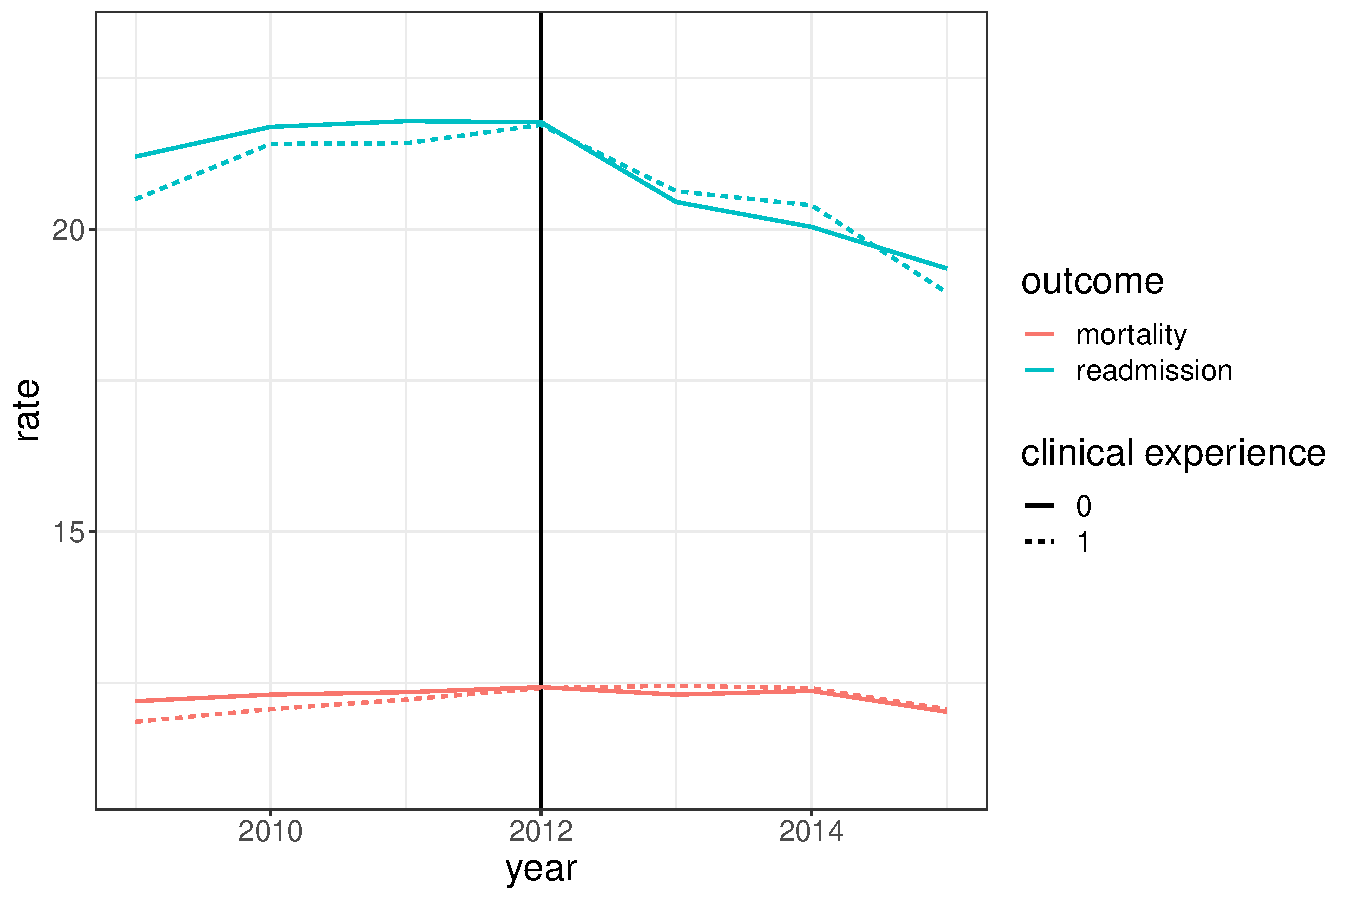
\includegraphics[width=\linewidth]{Objects/weighted_read_mort_graph.pdf}
    \end{figure}

    \hyperlink{sumstats}{\beamerbutton{stats}}
\end{frame}

\begin{frame}{Estimation Strategy}

    Compare hospitals with and without clinical experience before and after penalties began:

    \vspace{3mm}
    
    \begin{equation*}
    y_{ht} = \alpha_{h} + \delta_t + \beta (clinical_h \times post\_penalty_{ht}) + \epsilon_{ht}
    \end{equation*}

    \vspace{10mm}\pause

    Identifying Assumptions:
    \begin{itemize}
        \item Before the penalty, clinical and non-clinical team hospitals trended similarly along quality dimensions
        \item Previously determined leadership team is exogenous to the financial shock
    \end{itemize}

    \vspace{5mm}

    Threat to identification would have to be a time-varying hospital characteristic correlated with both clinical experience and outcomes
\end{frame}

\begin{frame}{All Hospital Response to Policy}\footnotesize
    \import{Tables}{policy_read_table.tex}
    \import{Tables}{policy_mort_table.tex}
\end{frame}


\begin{frame}{Differential Response in Readmissions}
   \small \import{Tables}{read_results_table.tex}
\end{frame}

\begin{frame}{Differential Response in Mortality}
    \small \import{Tables}{mort_results_table.tex}
\end{frame}

\begin{frame}{Conclusion}
\begin{wideitemize}
    \item While non-clinical teams have higher readmission rates before the penalty, they decrease readmissions at a faster rate after the penalties, though the effect is small
    \item No difference in mortality response
\end{wideitemize}

\vspace{10mm}

Now the question is why? 
\begin{itemize}
    \item Are non-clinical teams adjusting patient mix? 
\end{itemize}
\end{frame}


\begin{frame}[noframenumbering]{}\label{execnames}
\hyperlink{clinexp}{\beamerbutton{back}}
\begin{tikzpicture}
\node (bad) {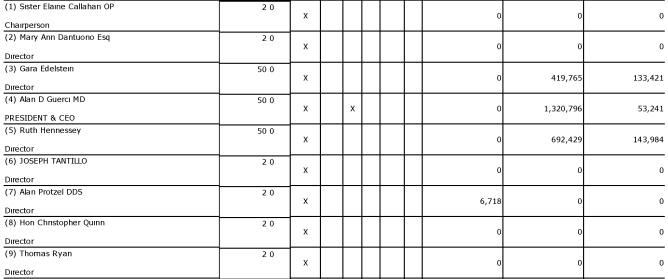
\includegraphics[scale=.5]{Graphics/990_snip_namesexample.PNG}};
\node (good) [right=of bad] {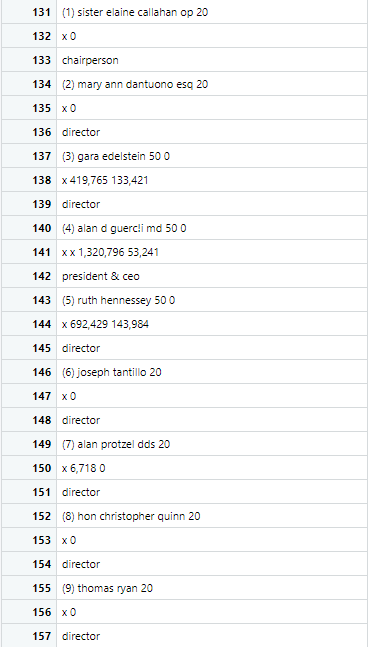
\includegraphics[scale=.45]{Graphics/r_snip_namesexample.PNG}};

\node (a) [fill=purple!50,draw] at (bad.center) {original pdf};
\node (b) [fill=purple!50,draw] at (good.center) {output from text extraction};

\draw [ultra thick,purple,->] (a) to[bend left] (b);
\end{tikzpicture}
\end{frame}

\begin{frame}[noframenumbering]{}\label{sumstats}
    \scriptsize \import{Tables}{sumstats_nooutcomes.tex}

    \hyperlink{sumstatsgraph}{\beamerbutton{back}}
\end{frame}





\end{document}